\documentclass[11pt]{article}
% \def\hidesolutions{}
%%%%%%%%%%% SET MARGINS
\setlength{\textheight}{20cm}
\setlength{\topmargin}{-0.5cm}
\setlength{\oddsidemargin}{+0cm}
\setlength{\textwidth}{16.3cm}
%\setlength{\parskip}{6pt}
\setlength{\parindent}{0pt}

%%%%%%%%%%% PACKAGES
\usepackage{amsmath}
\usepackage{amssymb}
\usepackage{amsfonts}
%\usepackage{a4wide}
\usepackage{graphicx}
\usepackage{color}
\usepackage[normalem]{ulem}
\usepackage{enumitem}
\usepackage{capt-of}
\usepackage{float}
\usepackage{amsmath}
\usepackage{listings}
\definecolor{mygreen}{RGB}{28,172,0} % color values Red, Green, Blue
\definecolor{mylilas}{RGB}{170,55,241}
\usepackage{empheq}
\usepackage[ruled]{algorithm2e}
\usepackage{mathrsfs}
\usepackage{datetime}
\usepackage{subcaption}

% TODO: combine the two package lists and reduce redundancies 
\usepackage{mathtools}
\usepackage{nicefrac}
\usepackage{hyperref}
\usepackage{url}
\usepackage{amsmath,amssymb,amsfonts}
\usepackage{a4wide}
\usepackage{graphicx}
\usepackage{color}
\usepackage[normalem]{ulem}
\usepackage{capt-of}
\usepackage{float}
\usepackage[ruled]{algorithm2e}
\usepackage{amsmath,amssymb,amsfonts}
\usepackage{a4wide}
\usepackage{graphicx}
\usepackage{color}
\usepackage[normalem]{ulem}
\usepackage{capt-of}
\usepackage{float}
\usepackage[ruled]{algorithm2e}
\usepackage{mathrsfs}







\newcommand{\Lc}[2]{{\color{blue} \sout{#1} } \textcolor{red}{#2}}
\newcommand{\La}[1]{\textcolor{red}{#1}}
\newcommand{\lh}{\mathscr{L}_h}
\newcommand{\cl}{\mathscr{L}}
\newcommand{\cf}{\mathscr{F}}
\newcommand{\dx}{dx}
\newcommand{\ltn}{\mathscr{l}^2}
\newcommand{\bbR}{\mathbb{R}}
\newcommand{\Rset}{\mathbb{R}}
\newcommand{\Nset}{\mathbb{N}}
\newcommand{\scL}{\mathcal{L}}
\newcommand{\xx}{\mathbf{x}}
\newcommand{\norm}[1]{\|{#1}\|}
\newcommand{\yy}{\mathbf{y}}
\newcommand{\at}[1]{\big|_{#1}}
\renewcommand{\div}{\mathrm{div}}
\newcommand{\divergence}{\mathrm{div}}
\newcommand{\cp}[1]{\textcolor{blue}{#1}}

\newcommand{\FF}{\texttt{FreeFem++ }}
\newcommand{\FFns}{\texttt{FreeFem++}}
\newcommand{\FFfull}{\texttt{FreeFem++-x11}}
\newcommand{\cmd}[1]{ \medskip \noindent \texttt{#1} \medskip}
\newcommand{\incmd}[1]{\texttt{#1}}
\newcommand{\shrinkitems}{\addtolength{\itemsep}{-0.5\baselineskip}}
\newcommand{\mtt}[1]{\mathtt{#1}}
\newcommand{\ML}{\texttt{Matlab }}

\newcommand{\bb}{\mathbf{b}}
\newcommand{\nn}{\mathbf{n}}
\newcommand{\vecA}{\vec{A}}
\newcommand{\vecB}{\vec{B}}


\newcommand{\mesh}{\mathcal{T}_h}
\newcommand{\refel}{\widehat{K}}
\newcommand{\ver}{\mathbf{a}}
\newcommand{\refver}{\widehat{\mathbf{a}}}
\newcommand{\grad}{\nabla}
\newcommand{\refgrad}{\widehat{\nabla}}
\newcommand{\refu}{\widehat{u}}
\newcommand{\refbasis}{\widehat{\varphi}}
\newcommand{\refxx}{\widehat{\xx}}
\newcommand{\refx}{\widehat{x}}
\newcommand{\refy}{\widehat{y}}
\newcommand{\refrho}{\widehat{\rho}}
\newcommand{\refh}{\widehat{h}}






% For typesetting Python code
\newcommand{\matlab}{{\sc Matlab}\xspace}
\usepackage{listings}
\lstloadlanguages{Python}
\lstloadlanguages{csh}%
\definecolor{MyDarkGreen}{rgb}{0.0,0.4,0.0}
\definecolor{purple}{rgb}{0.58,0,0.82}
\lstset{language=Python,                    % Use Python
	%frame=single,                          % Single frame around code
	basicstyle=\ttfamily\footnotesize\color{black},
	keywordstyle=[1]\color{blue}\bf,        % Python functions bold and blue
	keywordstyle=[2]\color{purple},         % Python function arguments purple
	keywordstyle=[3]\color{red}\underbar,   % User functions underlined and blue
	commentstyle=\usefont{T1}{pcr}{m}{sl}\color{MyDarkGreen}\small,
	stringstyle=\color{purple},
	showstringspaces=false,                 % Don't put marks in string spaces
	tabsize=3,                              % 5 spaces per tab
	morekeywords={xlim,ylim,var,alpha,factorial,poissrnd,normpdf,normcdf},
	morecomment=[l][\color{blue}]{...},
	breaklines=true,
	breakatwhitespace=true,
	emptylines=1,
	mathescape=true,
	xleftmargin=0ex,
	emphstyle=\bfseries\color{red}
}





%%%%%%%%%%% MACROS NAMES
\newcommand{\lecturername}{Martin Licht}
% \newcommand{\assistantnamea}{Jochen Hinz}
% \newcommand{\assistantnameb}{Ivan Bioli}
\newcommand{\semestername}{Winter Semester 2023}
\newcommand{\lecturename}{Analysis III - 202(c)}
\DeclarePairedDelimiter\floor{\lfloor}{\rfloor}

%%%%%%%%%%% HEADER
\newdateformat{yeardate}{\THEYEAR}
\newcommand{\exsheet}[3] % input is the number of the session and the day TODO What's that
{\clearpage

	\begin{center}
		{\Large \textbf{\lecturename}}\\[2ex]
		\semestername
	\end{center}

	% \vspace{2ex}
	% \lecturername

	\vspace{2ex}
	{\Large Session #1: #3\,#2, \yeardate\today}
	%\hfill
	%{\Large EPF Lausanne}

	\hrulefill
}





\usepackage{comment}

\newtheorem{exercise}{Exercise}
\newtheorem{solutionenv}{Solution}

\newboolean{hide_solution}
\ifx\hidesolutions\undefined
\newenvironment{solution}{\begin{solutionenv}}{\end{solutionenv}}
\setboolean{hide_solution}{false}
\else
\excludecomment{solution}
\setboolean{hide_solution}{true}
\fi

\newcommand{\ifnotsolution}[1]{\ifthenelse{\boolean{hide_solution}}{#1}{}}
\newcommand{\ifsolution}[1]{\ifthenelse{\boolean{hide_solution}}{}{#1}}








\allowdisplaybreaks

\begin{document}
\exsheet{14}{19}{December} % parameters are the number of the session and the day








%%%%%%%%%%%%%%%%%%%%%%%%%%%%%%%%%%%%%%%%%%%%%%%%%%%%%%%%
%%%%%%%%%%%%%%%%%%%%%%%%%%%%%%%%%%%%%%%%%%%%%%%%%%%%%%%%
%%%%%%%%%%%%%%%%%%%%%%%%%%%%%%%%%%%%%%%%%%%%%%%%%%%%%%%%
%%%%%                                        %%%%%%%%%%%
%%%%%   EXERCISE 1                           %%%%%%%%%%%
%%%%%                                        %%%%%%%%%%%
%%%%%%%%%%%%%%%%%%%%%%%%%%%%%%%%%%%%%%%%%%%%%%%%%%%%%%%%
%%%%%%%%%%%%%%%%%%%%%%%%%%%%%%%%%%%%%%%%%%%%%%%%%%%%%%%%
%%%%%%%%%%%%%%%%%%%%%%%%%%%%%%%%%%%%%%%%%%%%%%%%%%%%%%%%
\begin{exercise}
    Given the following functions over an interval $[0,1)$, 
    \begin{enumerate}[label=(\alph*)]
        \item $f(x) = x$
        \item $g(x) = x^2$
        \item $h(x) = e^x$
        \item $s(x) = sin(\pi x)$
    \end{enumerate}
    sketch their extension to 
    \begin{itemize}
        \item a periodic function with period $1$,
        \item an even periodic function with period $2$,
        \item an odd periodic function with period $2$.
    \end{itemize}
    State the formulas for the even and odd $2$-periodic extensions over the interval $[-1,1]$.
\end{exercise}

\begin{solution}
    We begin with these plots:
    \begin{center}
        \begin{tabular}{cc} % 2x2 matrix structure
            \begin{tikzpicture}[scale=0.6]
                \draw[->] (-2,0)--(2,0) node[right]{$x$};
                \draw[->] (0,-3)--(0,3) node[above]{$y$};
                \draw[domain=-2:-1,smooth,variable=\x,blue] plot({\x},{\x+2});
                \draw[domain=-1:0,smooth,variable=\x,blue] plot({\x},{\x+1});
                \draw[domain=0:1,smooth,variable=\x,blue] plot({\x},{\x});
                \draw[domain=1:2,smooth,variable=\x,blue] plot({\x},{\x-1});
                \node[blue,above right] at (0.5,0.5) {$f(x)=x$};
            \end{tikzpicture}
            &
            \begin{tikzpicture}[scale=0.6]
                \draw[->] (-2,0)--(2,0) node[right]{$x$};
                \draw[->] (0,-3)--(0,3) node[above]{$y$};
                \draw[domain=-2:-1,smooth,variable=\x,red] plot({\x},{(\x+2)*(\x+2)});
                \draw[domain=-1:0,smooth,variable=\x,red] plot({\x},{(\x+1)*(\x+1)});
                \draw[domain=0:1,smooth,variable=\x,red] plot({\x},{\x*\x});
                \draw[domain=1:2,smooth,variable=\x,red] plot({\x},{(\x-1)*(\x-1)});
                \node[red,above] at (0.5,0.5) {$g(x)=x^2$};
            \end{tikzpicture}
            \\
            \begin{tikzpicture}[scale=0.6]
                \draw[->] (-2,0)--(2,0) node[right]{$x$};
                \draw[->] (0,-3)--(0,3) node[above]{$y$};
                \draw[domain=-2:-1,smooth,variable=\x,green] plot({\x},{exp(\x+2)});
                \draw[domain=-1:0,smooth,variable=\x,green] plot({\x},{exp(\x+1)});
                \draw[domain=0:1,smooth,variable=\x,green] plot({\x},{exp(\x)});
                \draw[domain=1:2,smooth,variable=\x,green] plot({\x},{exp(\x-1)});
                \node[green,above right] at (0.5,1.5) {$h(x)=e^x$};
            \end{tikzpicture}
            &
            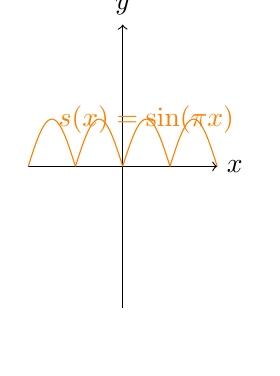
\begin{tikzpicture}[scale=0.6]
                \draw[->] (-2,0)--(2,0) node[right]{$x$};
                \draw[->] (0,-3)--(0,3) node[above]{$y$};
                \draw[domain=-2:-1,smooth,variable=\x,orange] plot({\x},{sin(3.14159*(\x+2) r)});
                \draw[domain=-1:0,smooth,variable=\x,orange] plot({\x},{sin(3.14159*(\x+1) r)});
                \draw[domain=0:1,smooth,variable=\x,orange] plot({\x},{sin(3.14159*\x r)});
                \draw[domain=1:2,smooth,variable=\x,orange] plot({\x},{sin(3.14159*(\x-1) r)});
                \node[orange,above] at (0.5,0.5) {$s(x)=\sin(\pi x)$};
            \end{tikzpicture}
        \end{tabular}
    \end{center}
    
    \begin{center}
        \begin{tabular}{cc} % 2x2 matrix structure
            \begin{tikzpicture}[scale=0.6]
                \draw[->] (-2,0)--(2,0) node[right]{$x$};
                \draw[->] (0,-3)--(0,3) node[above]{$y$};
                \draw[domain=-1:1,smooth,variable=\x,blue] plot({\x},{abs(\x)});
                \draw[domain=1:2,smooth,variable=\x,blue] plot({\x},{abs(\x-2)});
                \draw[domain=-2:-1,smooth,variable=\x,blue] plot({\x},{abs(\x+2)});
                \node[blue,above right] at (0.5,0.5) {$f_{\text{even}}(x)$};
            \end{tikzpicture}
            &
            \begin{tikzpicture}[scale=0.6]
                \draw[->] (-2,0)--(2,0) node[right]{$x$};
                \draw[->] (0,-3)--(0,3) node[above]{$y$};
                \draw[domain=-1:1,smooth,variable=\x,red] plot({\x},{\x*\x});
                \draw[domain=1:2,smooth,variable=\x,red] plot({\x},{abs(\x-2)*abs(\x-2)});
                \draw[domain=-2:-1,smooth,variable=\x,red] plot({\x},{abs(\x+2)*abs(\x+2)});
                \node[red,above] at (0.5,0.5) {$g_{\text{even}}(x)$};
            \end{tikzpicture}
            \\
            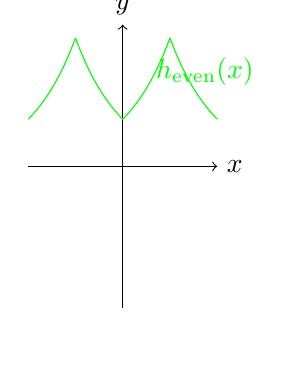
\begin{tikzpicture}[scale=0.6]
                \draw[->] (-2,0)--(2,0) node[right]{$x$};
                \draw[->] (0,-3)--(0,3) node[above]{$y$};
                \draw[domain=-1:1,smooth,variable=\x,green] plot({\x},{exp(abs(\x))});
                \draw[domain=1:2,smooth,variable=\x,green] plot({\x},{exp(abs(\x-2))});
                \draw[domain=-2:-1,smooth,variable=\x,green] plot({\x},{exp(abs(\x+2))});
                \node[green,above right] at (0.5,1.5) {$h_{\text{even}}(x)$};
            \end{tikzpicture}
            &
            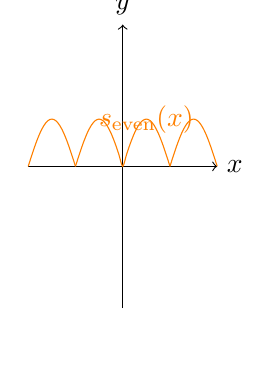
\begin{tikzpicture}[scale=0.6]
                \draw[->] (-2,0)--(2,0) node[right]{$x$};
                \draw[->] (0,-3)--(0,3) node[above]{$y$};
                \draw[domain=-1:1,smooth,variable=\x,orange] plot({\x},{sin(3.14159*abs(\x) r)});
                \draw[domain=1:2,smooth,variable=\x,orange] plot({\x},{sin(3.14159*abs(\x-2) r)});
                \draw[domain=-2:-1,smooth,variable=\x,orange] plot({\x},{sin(3.14159*abs(\x+2) r)});
                \node[orange,above] at (0.5,0.5) {$s_{\text{even}}(x)$};
            \end{tikzpicture}
        \end{tabular}
    \end{center}

    \begin{center}
        \begin{tabular}{cc} % 2x2 matrix structure
            \begin{tikzpicture}[scale=0.6]
                \draw[->] (-2,0)--(2,0) node[right]{$x$};
                \draw[->] (0,-3)--(0,3) node[above]{$y$};
                \draw[domain=-1:1,smooth,variable=\x,blue] plot({\x},{\x});
                \draw[domain=1:2,smooth,variable=\x,blue] plot({\x},{\x-2});
                \draw[domain=-2:-1,smooth,variable=\x,blue] plot({\x},{\x+2});
                \node[blue,above right] at (0.5,0.5) {$f_{\text{odd}}(x)$};
            \end{tikzpicture}
            &
            \begin{tikzpicture}[scale=0.6]
                \draw[->] (-2,0)--(2,0) node[right]{$x$};
                \draw[->] (0,-3)--(0,3) node[above]{$y$};
                \draw[domain=-2:-1,smooth,variable=\x,red] plot({\x}, {(\x+2)*(\x+2)});
                \draw[domain=-1: 0,smooth,variable=\x,red] plot({\x},-{\x*\x});
                \draw[domain= 0: 1,smooth,variable=\x,red] plot({\x}, {\x*\x});
                \draw[domain= 1: 2,smooth,variable=\x,red] plot({\x},-{(\x-2)*(\x-2)});
                \node[red,above] at (0.5,0.5) {$g_{\text{odd}}(x)$};
            \end{tikzpicture}
            \\
            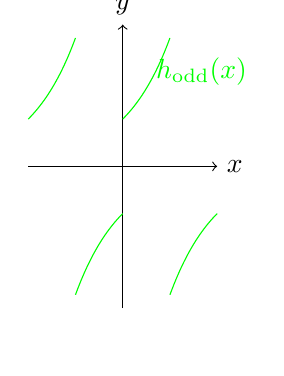
\begin{tikzpicture}[scale=0.6]
                \draw[->] (-2,0)--(2,0) node[right]{$x$};
                \draw[->] (0,-3)--(0,3) node[above]{$y$};
                \draw[domain=-2:-1,smooth,variable=\x,green] plot({\x}, {exp( \x+2)});
                \draw[domain=-1: 0,smooth,variable=\x,green] plot({\x},-{exp(-\x  )});
                \draw[domain= 0: 1,smooth,variable=\x,green] plot({\x}, {exp( \x  )});
                \draw[domain= 1: 2,smooth,variable=\x,green] plot({\x},-{exp(-\x+2)});
                \node[green,above right] at (0.5,1.5) {$h_{\text{odd}}(x)$};
            \end{tikzpicture}
            &
            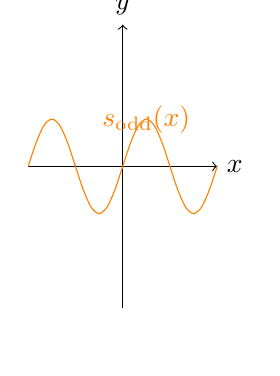
\begin{tikzpicture}[scale=0.6]
                \draw[->] (-2,0)--(2,0) node[right]{$x$};
                \draw[->] (0,-3)--(0,3) node[above]{$y$};
                \draw[domain=-2:2,smooth,variable=\x,orange] plot({\x},{sin(3.14159*\x r)});
                \node[orange,above] at (0.5,0.5) {$s_{\text{odd}}(x)$};
            \end{tikzpicture}
        \end{tabular}
    \end{center}
    We state the formulas for the even and odd extensions of period $2$.
    Over \([-1,1]\), define the even extensions:
    \begin{align*}
        f_{\text{even}}(x) &= |x|, 
        \\
        g_{\text{even}}(x) &= x^2,
        \\
        h_{\text{even}}(x) &= e^{|x|}, 
        \\
        s_{\text{even}}(x) &= |\sin(\pi x)|,
    \end{align*}
    and we define the odd extensions:
    \begin{align*}
        f_{\text{odd}}(x) &= x, 
        \\
        g_{\text{odd}}(x) &= \begin{cases}
        x^2 & x \in [0,1) \\
        -(-x)^2 = -x^2 & x \in [-1,0)
        \end{cases}
        \\
        h_{\text{odd}}(x) &= \begin{cases}
        e^x & x \in [0,1) \\
        -e^{-x} & x \in [-1,0)
        \end{cases}, 
        \\
        s_{\text{odd}}(x) &= \sin(\pi x).
    \end{align*}
\end{solution}



%%%%%%%%%%%%%%%%%%%%%%%%%%%%%%%%%%%%%%%%%%%%%%%%%%%%%%%%
%%%%%%%%%%%%%%%%%%%%%%%%%%%%%%%%%%%%%%%%%%%%%%%%%%%%%%%%
%%%%%%%%%%%%%%%%%%%%%%%%%%%%%%%%%%%%%%%%%%%%%%%%%%%%%%%%
%%%%%                                        %%%%%%%%%%%
%%%%%   EXERCISE 2                           %%%%%%%%%%%
%%%%%                                        %%%%%%%%%%%
%%%%%%%%%%%%%%%%%%%%%%%%%%%%%%%%%%%%%%%%%%%%%%%%%%%%%%%%
%%%%%%%%%%%%%%%%%%%%%%%%%%%%%%%%%%%%%%%%%%%%%%%%%%%%%%%%
%%%%%%%%%%%%%%%%%%%%%%%%%%%%%%%%%%%%%%%%%%%%%%%%%%%%%%%%
\begin{exercise}
    Consider the function 
    \begin{align*}
        f : [0,1] \to \bbR, \quad x \mapsto x^{3}.
    \end{align*}
    Extend this to an odd function with period $T = 2$. Sketch the graph of that function from $-2$ to $2$.
    Compute its Fourier coefficients in standard form. Compute the complex Fourier coefficients.
\end{exercise}
\begin{solution}
    We first sketch the odd extensions of that function:
    \begin{center}
    \begin{tikzpicture}[scale=0.6]
        \draw[->] (-2,0)--(2,0) node[right]{$x$};
        \draw[->] (0,-3)--(0,3) node[above]{$y$};
        % g(x) = x^3, odd extension
        \draw[domain=-2:-1,smooth,variable=\x,red] plot({\x}, {(\x+2)*(\x+2)*(\x+2)});
        \draw[domain=-1: 0,smooth,variable=\x,red] plot({\x}, {\x*\x*\x});
        \draw[domain= 0: 1,smooth,variable=\x,red] plot({\x}, {\x*\x*\x});
        \draw[domain= 1: 2,smooth,variable=\x,red] plot({\x}, {(\x-2)*(\x-2)*(\x-2)});

        \node[red,above] at (0.5,0.5) {$g_{\text{odd}}(x)$};
    \end{tikzpicture}
    \end{center}
    The odd extension of period 2 is given by
    \begin{align*}
        f_{\text{odd}}(x) = x^3, \quad x \in [-1,1].
    \end{align*}
    For the Fourier coefficients in standard form, we note that $a_n = 0, n \in \mathbb{N}$ since the function is odd by construction. For the sine-terms, we have
    \begin{align*}
        b_n = \int_{-1}^1 f_{\text{odd}}(x) \sin(\pi n x) \ dx = 2 \int_{0}^1 x^3 \sin(\pi n x) \ dx 
        = \frac{2(-1)^n (6 - \pi^2 n^2)}{\pi^3 n^3}.
    \end{align*}
    We directly compute the integral via repeated integration by parts:
    \begin{align*}
        \int_{0}^1 x^3 \sin(\pi n x) \ dx
        &
        =
        \left[ x^3 \tfrac{(-1)}{\pi n} \cos(\pi n x)\right]_{x=0}^{x=1}
        + 
        3 \tfrac{(-1)}{\pi n} \int_{0}^1 x^2 \cos(\pi n x) \ dx
        \\&
        =
        \tfrac{(-1)}{\pi n} \cos(\pi n) 
        + 
        3 \tfrac{(-1)}{\pi n} \int_{0}^1 x^2 \cos(\pi n x) \ dx
        \\&
        =
        - \tfrac{(-1)^{n}}{\pi n} 
        + 
        3 \tfrac{(-1)}{\pi n} \int_{0}^1 x^2 \cos(\pi n x) \ dx
        .
    \end{align*}
    \begin{align*}
        \int_{0}^1 x^2 \cos(\pi n x) \ dx
        =
        \left[ x^2 \tfrac{1}{\pi n} \sin(\pi n x)\right]_{x=0}^{x=1} 
        + 
        2 \tfrac{1}{\pi n} \int_{0}^1 x \sin(\pi n x) \ dx
        =
        2 \tfrac{1}{\pi n} \int_{0}^1 x \sin(\pi n x) \ dx
        .
    \end{align*}
    \begin{align*}
        \int_{0}^1 x \sin(\pi n x) \ dx
        &
        =
        \left[ x \tfrac{(-1)}{\pi n} \cos(\pi n x)\right]_{x=0}^{x=1}
        +
        \tfrac{(-1)}{\pi n}
        \int_{0}^1 \cos(\pi n x) \ dx
        \\& 
        =
        \left[ x \tfrac{(-1)}{\pi n} \cos(\pi n x)\right]_{x=0}^{x=1}
        +
        \tfrac{1}{\pi^{2} n^{2}}
        \left[ \sin(\pi n x)\right]_{x=0}^{x=1}
        \\& 
        =
        (-1)^{n}
        \tfrac{(-1)}{\pi n}
        .
    \end{align*}
    Putting all this together, we obtain 
    \begin{align*}
        \int_{0}^1 x^3 \sin(\pi n x) \ dx
        &
        =
        - \tfrac{(-1)^{n}}{\pi n} 
        + 
        3 \tfrac{(-1)}{\pi n} 
        2 \tfrac{1}{\pi n} 
        (-1)^{n}
        \tfrac{(-1)}{\pi n}
        \\&
        =
        - \frac{(-1)^{n}}{\pi n} 
        + 
        \frac{6}{\pi^{3} n^{3}} 
        (-1)^{n}
        \\&
        =
        (-1)^{n}
        \frac{ \pi^{2} n^{2} - 6 }{ \pi^{3} n^{3} }
        .
    \end{align*}


    For the complex Fourier coefficients, we find for $n \in \mathbb{N}$:
    \begin{align*}
        c_0 &= a_0 = 0,
        \\
        c_n &= \frac 1 2 (a_n - i b_n) = \frac{i (-1)^{n+1} (\pi^2 n^2 - 6)}{\pi^3 n^3},
        \\
        c_{-n} &= \frac 1 2 (a_n + i b_n) = \frac{i(-1)^n(\pi^2 n^2 - 6)}{\pi^3 n^3}.
    \end{align*}
    
\end{solution}







%%%%%%%%%%%%%%%%%%%%%%%%%%%%%%%%%%%%%%%%%%%%%%%%%%%%%%%%
%%%%%%%%%%%%%%%%%%%%%%%%%%%%%%%%%%%%%%%%%%%%%%%%%%%%%%%%
%%%%%%%%%%%%%%%%%%%%%%%%%%%%%%%%%%%%%%%%%%%%%%%%%%%%%%%%
%%%%%                                        %%%%%%%%%%%
%%%%%   EXERCISE 3                           %%%%%%%%%%%
%%%%%                                        %%%%%%%%%%%
%%%%%%%%%%%%%%%%%%%%%%%%%%%%%%%%%%%%%%%%%%%%%%%%%%%%%%%%
%%%%%%%%%%%%%%%%%%%%%%%%%%%%%%%%%%%%%%%%%%%%%%%%%%%%%%%%
%%%%%%%%%%%%%%%%%%%%%%%%%%%%%%%%%%%%%%%%%%%%%%%%%%%%%%%%
\begin{exercise}
    Suppose that
    \begin{align*}
        f(x) = \left\{\begin{array}{cc} x+1 & \text{ if $-1 < x < 0$ }, \\  1-x & \text{ if $ 0 < x < 1$ }, \\  0 & \text{ otherwise. } \end{array}\right.
        \qquad 
        g(x) = \left\{\begin{array}{cc} \frac 1 2 & \text{ if $-1 < x < 1$ }, \\ 0 & \text{ otherwise. } \end{array}\right.
        \qquad 
        h(x) = |x|
        .
    \end{align*}
    Compute the convolutions $u(x) = (f \star g)(x)$ and $v(x) = (g \star g)(x)$ and $w(x) = (g \star h)(x)$.
\end{exercise}
\begin{solution}
    We can compute these convolutions via direct computations or by results from Fourier analysis.
    \begin{itemize}
        \item 
        This first one is the most difficult one. First, we note that
        \begin{align*}
            g(x) = \frac 1 2 1_{[-1,1]}(x), & & 1_{[-1,1]}(x) = \begin{cases}
                1 & x \in [-1,1],\\
                0 & \text{otherwise},
            \end{cases}
        \end{align*}
        and
        \begin{align*}
            f(x) = (x+1) 1_{[-1,0]}(x) + (1-x) 1_{(0,1]}(x).
        \end{align*}
        Furthermore, we have for any $x, y \in \mathbb R$ that
        \begin{align*}
            1_{[-1, 1]}(x - y) &= 1_{[x - 1, x + 1]}(y).
        \end{align*}
        Hence, we can write
        \begin{align*}
            ( f \star g )(x) &= \frac 1 2 \int_{-\infty}^\infty f(y) 1_{[x - 1, x + 1]}(y) dy.
        \end{align*}
        We think of this as a subinterval $[x-1,x+1]$ that moves over the real line, 
        and we integrate $f$ over this subinterval. 
        Since $f$ change its behavior three different times, the integral in the definition of $f \star g$ above will also change its behavior several times, depending on $x$.
        
        We therefore use a case distinction. 
        \begin{enumerate}
            \item If $x < -2$, the integral is just over the region where $f$ equals zero,
            and so $( f \star g )(x) = 0$.
            \item If $-2 < x < -1$, then we only need to integrate $f$ over $[-1,x+1] \subseteq [-1,0]$. We find 
            \begin{align*}
                (f \star g)(x) = \frac 1 2 \int_{-1}^{x + 1} (y + 1) dy = \frac 1 4 (x + 2)^2.
            \end{align*}
            \item If $-1 < x < 0$, then we integrate $f$ over $[-1,0] \cup [0,x+1] \subseteq [-1,1]$. We find 
            \begin{align*}
                (f \star g)(x) = \frac 1 2\int_{-1}^{0} (y + 1) dy + \frac 1 2\int_{0}^{x + 1} (1 - y) dy =  \frac 1 2 - \frac 1 4 x^2.
            \end{align*}
            \item If $0 < x < 1$, then we integrate $f$ over $[x-1,0] \cup [0,1] \subseteq [-1,1]$. We find 
            \begin{align*}
                (f \star g)(x) = \frac 1 2 \int_{x - 1}^{0} (y + 1) dy + \frac 1 2 \int_{0}^{1} (1 - y) dy = \frac 1 2 - \frac 1 4 x^2.
            \end{align*}
            \item If $1 < x < 2$, then we integrate $f$ over $[x-1,1] \subseteq [0,1]$. We find 
            \begin{align*}
                (f \star g)(x) = \frac 1 2 \int_{x - 1}^{1} (1 - y) dy = \frac 1 4 ( x - 2)^2
            \end{align*}
            \item Lastly, if $2 < x$, the integral is just over the region where $f$ equals zero, 
            and so $( f \star g )(x) = 0$.
        \end{enumerate}


        
        \item 
        Note that
        \begin{align*}
            \hat{f}(\omega) &= \frac{1}{\sqrt{2 \pi}} \left(\frac{\sin(\omega / 2)}{\omega / 2}\right),
            \\
            \hat{g}(\omega) &= \frac{1}{\sqrt{2 \pi}} \frac{\sin(\omega)}{\omega}.
        \end{align*}
        Using the Convolution Theorem, we find
        \begin{align*}
            \hat{v}(\omega) = \sqrt{2 \pi}(\hat g (\omega))^2 = \hat f(2 \omega)
        \end{align*}
        Using the Modulation Theorem, we find
        \begin{align*}
            v(x) &= \frac 1 2 \mathcal{F}^{-1}(2 \hat f(2 \omega)) = \frac 1 2 f(\frac x 2)\\
                &= \frac 1 4 \begin{cases}
                    2 + x,& -2 \leq x < 0,\\
                    2 - x,& 0 \leq x < 2.
                \end{cases}
        \end{align*}
        Alternatively, consider 
        \begin{align*}
            ( g \star g )(x) = \frac 1 2 \int_{x-1}^{x+1} g(y) \ dy.
        \end{align*}
        Clearly, this equals $0$ when $x < -2$ or when $x > 2$ because then $(x-1,x+1)$ and $(-1,1)$ are disjoint. 
        So it remains to consider the case $-2 < x < 2$.
        The integral equals (up to a factor of $\tfrac 1 2$, the length of the intersection of $(x-1,x+1)$ and $(-1,1)$. 
        To put this into a formula, it seems reasonable to distinguish whether $x$ lies to the left or to the right of the origin.
        If $-1 \leq x \leq 0$, then 
        \begin{align*}
            \int_{x-1}^{x+1} g(y) \ dy = \int_{-1}^{x+1} g(y) \ dy = \frac 1 2 ( (x+1) - (-1) ) = \frac 1 2 ( x + 2 ).
        \end{align*}
        Hence 
        \begin{align*}
            ( g \star g )(x) = \frac 1 4 ( x + 2 ).
        \end{align*}
        If $0 \leq x \leq 1$, then 
        \begin{align*}
            \int_{x-1}^{x+1} g(y) \ dy = \int_{x-1}^{1} g(y) \ dy = \frac 1 2 ( (1) - (x-1) ) = \frac 1 2 ( 2 - x ).
        \end{align*}
        Hence 
        \begin{align*}
            ( g \star g )(x) = \frac 1 4 ( 2 - x ).
        \end{align*}
        
        \item 
        We first observe 
        \begin{align*}
            ( g \star h )(x) = \frac 1 2 \int_{x-1}^{x+1} |y| dy.
        \end{align*}
        From here, we make a case distinction. 
        If $0 < x-1$, which means $1 < x$, then 
        \begin{align*}
            ( g \star h )(x) =   \frac 1 2 \int_{x-1}^{x+1}    y dy =  x.
        \end{align*}
        If $x+1 < 0$, which means $x < -1$, then 
        \begin{align*}
            ( g \star h )(x) =   \frac 1 2 \int_{x-1}^{x+1} (-y) dy = -x.
        \end{align*}
        The case $x-1 < 0 < x+1$, which is $-1 < x < 1$, is more demanding. We split 
        \begin{align*}
            ( g \star h )(x) 
            &= 
            \frac 1 2 \int_{x-1}^{  0} -y dy
            +
            \frac 1 2 \int_{  0}^{x+1}  y dy
            \\&
            =
            \frac 1 2 \left[ -\frac 1 2 y^{2}\right]_{y=x-1}^{y=  0}
            +
            \frac 1 2 \left[  \frac 1 2 y^{2}\right]_{y=  0}^{y=x+1}
            \\&
            =
            \frac 1 4 (x-1)^{2} 
            +
            \frac 1 4 (x+1)^{2} 
            =
            \frac 1 2 x^2 + \frac 1 2
            .
        \end{align*}
        Note: if you plot this function, it will look like a moving average of $|x|$ that has been smoothed around $x=0$.
    \end{itemize}
\end{solution}



%%%%%%%%%%%%%%%%%%%%%%%%%%%%%%%%%%%%%%%%%%%%%%%%%%%%%%%%
%%%%%%%%%%%%%%%%%%%%%%%%%%%%%%%%%%%%%%%%%%%%%%%%%%%%%%%%
%%%%%%%%%%%%%%%%%%%%%%%%%%%%%%%%%%%%%%%%%%%%%%%%%%%%%%%%
%%%%%                                        %%%%%%%%%%%
%%%%%   EXERCISE 4                           %%%%%%%%%%%
%%%%%                                        %%%%%%%%%%%
%%%%%%%%%%%%%%%%%%%%%%%%%%%%%%%%%%%%%%%%%%%%%%%%%%%%%%%%
%%%%%%%%%%%%%%%%%%%%%%%%%%%%%%%%%%%%%%%%%%%%%%%%%%%%%%%%
%%%%%%%%%%%%%%%%%%%%%%%%%%%%%%%%%%%%%%%%%%%%%%%%%%%%%%%%
\begin{exercise}
    Suppose that $f(x) = x^2$ and that
    \begin{align*}
        g(x) = \left\{\begin{array}{cc} \frac 1 2 & \text{ if $-1 < x < 1$ }, \\ 0 & \text{ otherwise. } \end{array}\right.
        \qquad 
        h(x) = \left\{\begin{array}{cc} e^{-x} & \text{ if $x > 0$ }, \\ 0 & \text{ otherwise. } \end{array}\right.
    \end{align*}
    Compute the convolutions $u(x) = (f \star g)(x)$ and $v(x) = (f \star h)(x)$ .
\end{exercise}

\begin{solution}
    We find by direct computation:
    \begin{align*}
        (f \star g)(x) = (g \star f)(x) = \frac 1 2 \int_{-1}^1 (x - y)^2 dy = x^2 + \frac 1 3.
    \end{align*}   
    Similarly,
    \begin{align*}
        (f \star h)(x) 
        = 
        \int_{0}^\infty (x - y)^2 e^{-y} dy 
        = 
        \int_{0}^\infty (y - x)^2 e^{-y} dy 
        .
    \end{align*}
    We proceed here with integration by parts: first, 
    \begin{align*}
        \int_{0}^\infty (y - x)^2 e^{-y} dy 
        &=
        \left[ - (y - x)^2 e^{-y} \right]_{y=0}^{y=\infty}
        -
        \int_{0}^\infty (-1)2(y - x) e^{-y} dy 
        \\
        &=
        x^2 
        +
        2
        \int_{0}^\infty (y - x) e^{-y} dy 
        .
    \end{align*}
    Then, 
    \begin{align*}
        \int_{0}^\infty (y - x) e^{-y} dy 
        &=
        \left[ - (y - x) e^{-y} \right]_{y=0}^{y=\infty}
        -
        \int_{0}^\infty (-1) e^{-y} dy 
        \\
        &=
        -x 
        +
        \int_{0}^\infty e^{-y} dy 
        .
    \end{align*}
    Lastly,
    \begin{align*}
        \int_{0}^\infty e^{-y} dy = \left[ - e^{-y} \right]_{y=0}^{y=\infty} = 1
        .
    \end{align*}
    Thus, in total, we obtain 
    \begin{align*}
        (f \star h)(x) 
        =
        x^{2} + 2 \left( -x + 1 \right) = x^{2} - 2 x + 2.
    \end{align*}
\end{solution}










%%%%%%%%%%%%%%%%%%%%%%%%%%%%%%%%%%%%%%%%%%%%%%%%%%%%%%%%
%%%%%%%%%%%%%%%%%%%%%%%%%%%%%%%%%%%%%%%%%%%%%%%%%%%%%%%%
%%%%%%%%%%%%%%%%%%%%%%%%%%%%%%%%%%%%%%%%%%%%%%%%%%%%%%%%
%%%%%                                        %%%%%%%%%%%
%%%%%   EXERCISE 5                           %%%%%%%%%%%
%%%%%                                        %%%%%%%%%%%
%%%%%%%%%%%%%%%%%%%%%%%%%%%%%%%%%%%%%%%%%%%%%%%%%%%%%%%%
%%%%%%%%%%%%%%%%%%%%%%%%%%%%%%%%%%%%%%%%%%%%%%%%%%%%%%%%
%%%%%%%%%%%%%%%%%%%%%%%%%%%%%%%%%%%%%%%%%%%%%%%%%%%%%%%%
\begin{exercise}
    We have discussed solutions to the differential equation 
    \begin{align*}
        - \Delta u(x) + k^2 u(x) = e^{-|x|}, \quad x \in \mathbb R.
    \end{align*}
    \begin{itemize}
        \item 
        Verify that, in the case $k=1$, we have a solution 
        \begin{align*}
            u(x) = \frac 1 2 (1+|x|) e^{-|x|} 
        \end{align*}
        Verify that every function of the form 
        \begin{align*}
            v(x) = \frac 1 2 (1+|x|) e^{-|x|} + c_1 e^{-x} + c_2 e^{x} 
        \end{align*}
        is a solution. For which values of $c_1$ and $c_2$ does the function decay towards zero as $x$ goes to $\pm \infty$?
        %
        \item 
        Verify that, in the case $k \neq 1$, we have a solution 
        \begin{align*}
            u(x) = - \frac{ e^{-k|x|} }{ k (k^2-1) } + \frac{ e^{-|x|} }{ k^2-1 }
        \end{align*}
        Verify that every function of the form 
        \begin{align*}
            v(x) = - \frac{ e^{-k|x|} }{ k (k^2-1) } + \frac{ e^{-|x|} }{ k^2-1 } + c_1 e^{-kx} + c_2 e^{kx} 
        \end{align*}        
        is a solution.
    \end{itemize}
\end{exercise}
\begin{solution}
    \begin{itemize}
    \item 
    Consider the function 
    \begin{align*}
        v(x) = \frac 1 2 (1+|x|) e^{-|x|} + c_1 e^{-x} + c_2 e^{x}.
    \end{align*}
    Obviously, $u(x)$ is a special case of a function of that form when $c_1 = c_2 = 0$. 
    This function is continuous and it is differentiable over $(-\infty,0)$ and $(0,\infty)$. 
    Its derivative equals 
    \begin{align*}
        v'(x) = - \frac 1 2 x e^{-|x|} - c_1 e^{-x} + c_2 e^{x}.
    \end{align*}
    To see that, we can, e.g., compute the $v'$ for $x > 0$ and $x < 0$ and verify that $v'$ matches this description. 
    
    This function is again continuous and it is differentiable over $(-\infty,0)$ and $(0,\infty)$. 
    Its derivative equals 
    \begin{align*}
        v''(x) = \frac 1 2 e^{-|x|} \left( |x| - 1 \right) + c_1 e^{-x} + c_2 e^{x}.
    \end{align*}
    That this is a solution to the differential equations is evident from 
    \begin{align*}
        - v''(x) + v(x) 
        &
        =
        - \frac 1 2 e^{-|x|} \left( |x| - 1 \right) -  c_1 e^{-x} - c_2 e^{x} + \frac 1 2 (1+|x|) e^{-|x|} + c_1 e^{-x} + c_2 e^{x}
        \\&
        =
        \frac 1 2 e^{-|x|} \left( 1 - |x| \right) + \frac 1 2 (1+|x|) e^{-|x|} 
        =
        e^{-|x|}
        .
    \end{align*}
    To ensure that the solution decays towards zero as $x$ goes to $\pm \infty$, we need to have $c_1 = c_2 = 0$.
    
    \item 
    We repeat the same type of arguments.
    Consider the function 
    \begin{align*}
        v(x) 
        &= 
        - \frac{ e^{-k|x|} }{ k (k^2-1) } 
        + 
        \frac{ e^{-|x|} }{ k^2-1 } 
        + 
        c_1 e^{-kx} 
        + 
        c_2 e^{kx}
        .
    \end{align*}
    Obviously, $u(x)$ is a special case of a function of that form when $c_1 = c_2 = 0$. 
    Clearly, $v$ is continuous and it is differentiable over $(-\infty,0)$ and $(0,\infty)$. 
    Calculations, for $v \neq 0$ show that the derivative (in the sense of distributions) equals 
    \begin{align*}
        v'(x)
        =
        \operatorname{sign}(x) \frac{ \left( e^{-k|x|} -  e^{-|x|} \right) }{ k^{2}-1 }
        + 
        (-k) c_1 e^{-kx} 
        + 
          k  c_2 e^{kx}
        .
    \end{align*}
    This function is still continuous and obviously differentiable over $(-\infty,0)$ and $(0,\infty)$. 
    We find that 
    \begin{align*}
        v''(x)
        &=
        2\delta_{0} \cdot \frac{ \left( e^{-k|x|} -  e^{-|x|} \right) }{ k^{2}-1 }
        +
        \operatorname{sign}(x)^{2} \frac{ \left( - k e^{-k|x|} + e^{-|x|} \right) }{ k^{2}-1 }
        + 
        k^{2} c_1 e^{-kx} 
        + 
        k^{2} c_2 e^{kx}
        \\&
        =
        \frac{ \left( - k e^{-k|x|} + e^{-|x|} \right) }{ k^{2}-1 }
        + 
        k^{2} c_1 e^{-kx} 
        + 
        k^{2} c_2 e^{kx}
        .
    \end{align*}
    Here, we have used that the $e^{-|x|} - e^{-k|x|} = 0$ at $x=0$. 
    
    That being settled, we check 
    \begin{align*}
        &
        - v''(x) + k^{2} v(x)
        \\&\qquad 
        =
        -
        \frac{ - k e^{-k|x|} + e^{-|x|} }{ k^{2}-1 }
        - 
        k^{2} c_1 e^{-x} 
        - 
        k^{2} c_2 e^{x}
        -
        k^{2} \frac{ e^{-k|x|} }{ k (k^2-1) } 
        + 
        k^{2} \frac{ e^{-|x|} }{ k^2-1 } 
        + 
        c_1 e^{-x} 
        + 
        c_2 e^{x}
        \\&\qquad 
        =
        \frac{ k e^{-k|x|} - e^{-|x|} }{ k^{2}-1 }
        - 
        \frac{ k e^{-k|x|} }{ (k^2-1) } 
        + 
        k^{2} \frac{ e^{-|x|} }{ k^2-1 } 
        \\&\qquad 
        =
        e^{-|x|}
        .
    \end{align*}
    This is the desired differential equation. 
    \end{itemize}
\begin{comment}
    We first note that the Fourier transform of $e^{-|x|}$ is given by
    \begin{align*}
        \mathcal F(e^{-|x|})(\omega) = \sqrt{\frac{2}{\pi}} \frac{1}{1+\omega^2}.
    \end{align*}
    Therefore, if $u(x)$ is a solution, then its Fourier transform $\hat u(\omega)$ satisfies
    \begin{align*}
        (\omega^2 + k^2) \hat u(\omega) = \sqrt{\frac{2}{\pi}} \frac{1}{1+\omega^2}.
    \end{align*}
    Therefore, if $k = 1$, then
    \begin{align*}
        \hat u(\omega) &= \sqrt{\frac{2}{\pi}} \frac{1}{(1+\omega^2)^2}\\
                    &= \mathcal{F}^{-1}(\frac{1}{2}(1 + |x|) e^{-|x|}).
    \end{align*}
    The last step can be seen from the results in the lecture.
    Thus, it is clear that $u(x) = \frac 1 2 (1+|x|) e^{-|x|}$ is a solution. Furthermore, 

    For the case $k \neq 1$, note that
    \begin{align*}
        \mathcal{F}(e^{-k|x|})(\omega) = \sqrt{\frac{2}{\pi}} \frac{k}{k^2 + \omega^2}.
    \end{align*}
    Therefore, the Fourier transform of the solution $u(x)$ satisfies
    \begin{align*}
        (\omega^2 + k^2) \hat u(\omega) &= \sqrt{\frac{2}{\pi}} (k^2 + \omega^2) \left[ \frac{-1}{(k^2 + \omega^2)(k^2 - 1)} + \frac{1}{(\omega^2 + 1)(k^2 - 1)} \right]
        \\
        &= \sqrt{\frac{2}{\pi}} (k^2 + \omega^2) \left[ \frac{k^2 -1}{(\omega^2 + 1)(k^2 - 1)(k^2 + \omega^2)} \right]
        \\
        &= \sqrt{\frac{2}{\pi}} \frac{1}{(1 + \omega^2)},
    \end{align*}
    as desired. The argument for the general solution is the same as for the case $k=1$.
\end{comment}
\end{solution}







%%%%%%%%%%%%%%%%%%%%%%%%%%%%%%%%%%%%%%%%%%%%%%%%%%%%%%%%
%%%%%%%%%%%%%%%%%%%%%%%%%%%%%%%%%%%%%%%%%%%%%%%%%%%%%%%%
%%%%%%%%%%%%%%%%%%%%%%%%%%%%%%%%%%%%%%%%%%%%%%%%%%%%%%%%
%%%%%                                        %%%%%%%%%%%
%%%%%   EXERCISE 6                           %%%%%%%%%%%
%%%%%                                        %%%%%%%%%%%
%%%%%%%%%%%%%%%%%%%%%%%%%%%%%%%%%%%%%%%%%%%%%%%%%%%%%%%%
%%%%%%%%%%%%%%%%%%%%%%%%%%%%%%%%%%%%%%%%%%%%%%%%%%%%%%%%
%%%%%%%%%%%%%%%%%%%%%%%%%%%%%%%%%%%%%%%%%%%%%%%%%%%%%%%%
\begin{exercise}
    We want to find a solution to the boundary value problem 
    \begin{gather*}
        - \Delta u(x) + k^2 u(x) = x, \quad 0 < x < L,
        \\
        u(0) = 0, \quad u(L) = 0.
    \end{gather*}
    \begin{itemize}
        \item Extend the right-hand side $f(x) = x$ to an odd function with period $2L$ and compute its Fourier coefficients.
        \item Using these coefficients, find the Fourier series of the solution $u$. Verify that the boundary condition $u(0) = u(L) = 0$ is satisfied.
    \end{itemize}
\end{exercise}
\begin{solution}
    \begin{itemize}
        \item The odd extension of period 2 is simply given by
        \begin{align*}
            f_{\mathrm{odd}}(x) = x, \quad x \in [-L,L].
        \end{align*}
        \item 
        Since $f_{\mathrm{odd}}$ is odd by construction, we have
        \begin{align*}
            f_{\mathrm{odd}}(x) = \sum_{n=1}^{\infty} f_n \sin(\frac{n \pi x}{L}),
        \end{align*}
        with
        \begin{align*}
            f_n 
            = 
            \frac{2}{L} \int_{0}^{L} x \sin(\frac{n \pi x}{L}) \ dx 
            &
            = 
            \frac{2}{L} 
            \left[ -x \frac{L}{n \pi} \cos\left( \frac{n \pi}{L} x \right) \right]_{x=0}^{x=L} 
            +
            \frac{2}{L} 
            \int_{0}^{L} \frac{L}{n \pi} \cos\left( \frac{n \pi}{L} x \right) \ dx 
            \\&
            = 
            \left[ -x \frac{2}{n \pi} \cos\left( \frac{n \pi}{L} x \right) \right]_{x=0}^{x=L} 
            +
            \frac{2}{n \pi} 
            \int_{0}^{L} \cos\left( \frac{n \pi}{L} x \right) \ dx 
            \\&
            = 
            \left[ -x \frac{2}{n \pi} \cos\left( \frac{n \pi}{L} x \right) \right]_{x=0}^{x=L} 
            +
            \frac{2}{n \pi} 
            \left[ \left( \frac{L}{n \pi} \right) \sin\left( \frac{n \pi}{L} x \right) \right]_{x=0}^{x=L} 
            \\&
            = 
            \left[ -x \frac{2}{n \pi} \cos\left( \frac{n \pi}{L} x \right) \right]_{x=0}^{x=L} 
            \\&
            = 
            -L \frac{2}{n \pi} \cos\left( n \pi \right)
            =
            (-1)^{n+1}\frac{2L}{\pi n}
            .
        \end{align*}
        \item 
        For the solution, we make a sine ansatz $u(x) = \sum_{n=1}^{\infty} u_n \sin(\frac{n \pi x}{L})$ 
        because this satisfies the boundary conditions. 
        Then, the PDE can be written in terms of the Fourier coefficients as
        \begin{align*}
            \left[ k^2 + \left(\frac{\pi n}{L} \right)^2 \right] u_n = (-1)^{n+1}\frac{2L}{\pi n}, & & \forall n \in \mathbb{N}.
        \end{align*}
        Therefore, the solution is given by
        \begin{align*}
            u_n 
            = 
            (-1)^{n+1}\frac{2L}{\pi n} 
            \left[ k^2 + \left(\frac{\pi n}{L} \right)^2 \right]^{-1}
            .
        \end{align*}
    \end{itemize}
\end{solution}































%%%%%%%%%%%%%%%%%%%%%%%%%%%%%%%%%%%%%%%%%%%%%%%%%%%%%%%%
%%%%%%%%%%%%%%%%%%%%%%%%%%%%%%%%%%%%%%%%%%%%%%%%%%%%%%%%
%%%%%%%%%%%%%%%%%%%%%%%%%%%%%%%%%%%%%%%%%%%%%%%%%%%%%%%%
%%%%%                                        %%%%%%%%%%%
%%%%%   EXERCISE 7                           %%%%%%%%%%%
%%%%%                                        %%%%%%%%%%%
%%%%%%%%%%%%%%%%%%%%%%%%%%%%%%%%%%%%%%%%%%%%%%%%%%%%%%%%
%%%%%%%%%%%%%%%%%%%%%%%%%%%%%%%%%%%%%%%%%%%%%%%%%%%%%%%%
%%%%%%%%%%%%%%%%%%%%%%%%%%%%%%%%%%%%%%%%%%%%%%%%%%%%%%%%
\begin{exercise}[Fun with Neumann boundary conditions]
    Consider the Poisson problem with \textit{Neumann boundary conditions} over the interval $[a,b] = [0,1]$: 
    \begin{gather*}
        - u''(x) + k^2 u(x) = x - \frac 1 2, \quad a < x < b,
        \\
        u'(a) = 0, \quad u'(b) = 0,
    \end{gather*}
    for some $k \geq 0$.
    \begin{enumerate}[label=(\alph*)]
        \item
        Extend $f(x) = x - \frac 1 2$ to an \textit{even} function over the real line with period $2$.
        \item 
        Compute the Fourier coefficients of that even extension of $f$.
        \item 
        Find the Fourier series of a function that satisfies the above differential equation.
    \end{enumerate}
\end{exercise}
\begin{solution}
    \begin{itemize}
        \item The even extension of period 2 is given by $f_{\text{even}}(x) = |x| - \frac 1 2, x \in [-1, 1]$.
        \item Since $f_{\text{even}}$ is even by construction, we only have cosine terms, i.e.
        \begin{align*}
            f_{\text{even}}(x) = \frac{f_0}{2} + \sum_{n=1}^{\infty} f_n \cos(\pi n x)
            .
        \end{align*}
        Here, 
        \begin{align*}
            f_0 = \frac{1}{2} \int_{-1}^{1} (|x| - \frac 1 2) \ dx = \int_{-1}^1 (x - \frac 1 2) \ dx = 0
            ,
        \end{align*}
        and for any $n \geq 1$,
        \begin{align*}
            f_n 
            &
            = 
              \int_{-1}^{1} (x- \frac 1 2) \cos(\pi n x) \ dx 
            \\&
            = 
            2 \int_{ 0}^{1} (x- \frac 1 2) \cos(\pi n x) \ dx 
            = 
            2 \int_{ 0}^{1} x \cos(\pi n x) \ dx 
            = 
            \frac{2}{\pi^2 n^2}\left( (-1)^n - 1 \right) % OKAY 7
            .
        \end{align*}
        \item 
        For the solution, we make a cosine ansatz 
        \begin{align*}
            u(x) = u_0 + \sum_{n=1}^{\infty} u_n \cos(\pi n x)
        \end{align*}
        because the cosine modes satisfy the Neumann boundary conditions. 
        We have expressed the (even extension) of the right-hand side as a Fourier cosine series,
        and therefore the PDE can be written in terms of the Fourier coefficients:
        \begin{align*}
            \left [k^2 + \pi^2 n^2 \right]u_n &= f_n = \frac{2}{\pi^2 n^2}\left( (-1)^n - 1 \right), & & \forall n \in \mathbb{N}.
        \end{align*}
        Note that no information can be provided for the coefficient $u_0$ when $k = 0$; indeed, any choice will be possible.\footnote{This corresponds to the fact that whenever we have solution of $-u'' = f$ with Neumann boundary conditions, then also $u+c$ is a solution to the same problem, for any constant $c \in \mathbb R$. In other words, the solution is not unique.} We have $u_0 = 0$. 
        
        This provides the coefficients of the Fourier (cosine) series of $u$:
        \begin{align*}
            u_n &= \left( k^2 + \pi^2 n^2 \right)^{-1} \frac{2}{\pi^2 n^2}\left( (-1)^n - 1 \right), & & \forall n \in \mathbb{N}.
        \end{align*}
        Therefore, the solution is given by 
        \begin{align*}
            u(x) = u_0 + \sum_{n=1}^{\infty} \frac{2}{\pi^2 n^2 \left[k^2 + \pi^2 n^2 \right]}\left( (-1)^n - 1 \right) \cos(\pi n x).
        \end{align*}
        The boundary conditions are satisfied by construction, because we have used a Fourier cosine series. 
    \end{itemize}
\end{solution}




















%%%%%%%%%%%%%%%%%%%%%%%%%%%%%%%%%%%%%%%%%%%%%%%%%%%%%%%%
%%%%%%%%%%%%%%%%%%%%%%%%%%%%%%%%%%%%%%%%%%%%%%%%%%%%%%%%
%%%%%%%%%%%%%%%%%%%%%%%%%%%%%%%%%%%%%%%%%%%%%%%%%%%%%%%%
%%%%%                                        %%%%%%%%%%%
%%%%%   EXERCISE 8                           %%%%%%%%%%%
%%%%%                                        %%%%%%%%%%%
%%%%%%%%%%%%%%%%%%%%%%%%%%%%%%%%%%%%%%%%%%%%%%%%%%%%%%%%
%%%%%%%%%%%%%%%%%%%%%%%%%%%%%%%%%%%%%%%%%%%%%%%%%%%%%%%%
%%%%%%%%%%%%%%%%%%%%%%%%%%%%%%%%%%%%%%%%%%%%%%%%%%%%%%%%

\begin{exercise}[Fun with periodic boundary conditions]
    Consider the Poisson problem with \textit{periodic boundary conditions} over the interval $[a,b] = [0,1]$: 
    \begin{gather*}
        - u''(x) + k^2 u(x) = x - \frac 1 2, \quad a < x < b,
        \\
        u(a) = u(b),
    \end{gather*}
    for some $k \geq 0$.
    \begin{enumerate}[label=(\alph*)]
        \item
        Extend $f(x) = x - \frac 1 2$ to a $1$-periodic function over the real line.
        \item 
        Compute the Fourier coefficients of that extension of $f$.
        \item 
        Find the Fourier series of a function that satisfies the above differential equation.
    \end{enumerate}
\end{exercise}
\begin{solution}
    \begin{enumerate}
        \item The $1$-periodic extension is simply given by $f_{\text{per}}(x) = x - \frac 1 2, x \in [0, 1]$ with periodic continuation.
        \item When we develop the Fourier coefficients of $f_{\text{per}}$, 
        \begin{align*}
            f_{\text{per}}(x) = \frac{a^{f}_0}{2} + \sum_{n \geq 1} a^{f}_{n} \cos( 2 \pi n x ) + b^{f}_{n} \sin( 2 \pi n x ).
        \end{align*}
        We note that $f_{\text{per}}$ happens to be an odd function, which means that $a^{f}_n = 0$ for $n \geq 0$,
        and it only remains to compute the sine coefficients:
        \begin{align*}
            f_{\text{per}}(x) = \sum_{n=1}^{\infty} b^{f}_n \sin(2 \pi n x),
        \end{align*}
        We compute the Fourier coefficients. We have 
        \begin{align*}
            b^{f}_n 
            &= 
            \int_{-1}^{1} \left( x- \frac 1 2 \right) \sin(2 \pi n x) \ dx 
            \\&= 
            2 
            \int_{ 0}^{1} \left( x- \frac 1 2 \right) \sin(2 \pi n x) \ dx 
            \\&= 
            2 
            \int_{ 0}^{1} x \sin(2 \pi n x) \ dx 
            - 
            \int_{ 0}^{1} \sin(2 \pi n x) \ dx 
            \\&= 
            2 
            \int_{ 0}^{1} x \sin(2 \pi n x) \ dx 
        \end{align*}
        Via integration by parts:
        \begin{align*}
            b^{f}_{n}
            = 
            2 
            \int_{ 0}^{1} x \sin(2 \pi n x) \ dx 
            &
            =
            2 
            \left[ x \frac{(-\cos)}{2\pi n}(2 \pi n x) \right]_{x=0}^{x=1}
            -
            \int_{0}^{1} \frac{(-\cos)}{2\pi n}(2 \pi n x) \ dx 
            \\&= 
            -
            2 
            \frac{1}{2\pi n}
            + 
            \frac{1}{2\pi n}
            \int_{0}^{1} \cos(2 \pi n x) \ dx 
            =
            \frac{-1}{\pi n}
%             = 
%             \int_{0}^{1} \left( x- \frac 1 2 \right) \sin(2 \pi n x) \ dx 
%             \\&
%             = 
%             \int_{0}^{1} x \sin(2 \pi n x) \ dx 
%             -
%             \int_{0}^{1} \sin(2 \pi n x) \ dx 
%             = 
%             \int_{0}^{1} x \sin(2 \pi n x) \ dx 
            .
        \end{align*}
%         Via integration by parts:
%         \begin{align*}
%             \int_{0}^{1} \left( x- \frac 1 2 \right) \sin(2 \pi n x) \ dx 
%             &
%             = 
%             \left[ x \frac{-1}{2 \pi n} \cos(2 \pi n x) \right]_{x=0}^{x=1}
%             -
%             \int_{0}^{1} \frac{-1}{2 \pi n} \cos(2 \pi n x) \ dx
%             \\&
%             = 
%             \left[ x \frac{-1}{2 \pi n} \cos(2 \pi n x) \right]_{x=0}^{x=1}
%             +
%             \frac{1}{ 4 \pi^{2} n^{2} } 
%             \left[ \sin( 2 \pi n x ) \right]_{x=0}^{x=1}
%             \\&
%             = 
%             \left[ x \frac{-1}{2 \pi n} \cos(2 \pi n x) \right]_{x=0}^{x=1}
%             \\&
%             = 
%             \frac{-1}{2 \pi n} \cos(2 \pi n) 
%             =
%             \frac{-1}{2 \pi n} 
%             .
%         \end{align*}

        \item 
        We use a full Fourier series for the solution of the Poisson problem with periodic boundary conditions,
        \begin{align*}
            u(x) = \frac{a^{u}_0}{2} + \sum_{n \geq 1} a^{u}_{n} \cos( 2 \pi n x ) + b^{u}_{n} \sin( 2 \pi n x ).
        \end{align*}
        because both the sine and cosine modes satisfy the periodic boundary conditions. 
        When we write the differential equation in terms of the Fourier coefficients, then we find that $a_0$ is indeterminate,\footnote{Similar 
        to the Neumann problem, if we have any solution to $-u'' = f$ with periodic boundary conditions, then so does $u+c$ for any constant $c \in \mathbb R$.} 
        and 
        \begin{align*}
            \left [k^2 + (2 \pi n)^2 \right] a^{u}_{n} = a^{f}_{n}, & & \forall n \in \mathbb{N}
            ,
            \\ 
            \left [k^2 + (2 \pi n)^2 \right] b^{u}_{n} = b^{f}_{n}, & & \forall n \in \mathbb{N}
            .
        \end{align*}
        With our specific choice of coefficients, 
        Therefore, the solution is given by
        \begin{align*}
            u(x) = \sum_{n=1}^{\infty} \frac{-1}{\pi n \left[k^2 + (2 \pi n)^2 \right]} \sin(2 \pi n x).
        \end{align*}
        Note that the periodic boundary conditions are satisfied.
    \end{enumerate}
\end{solution}



% \begin{exercise}
% \end{exercise}
% \begin{solution}     
% \end{solution}
% 
% \begin{exercise}
% \end{exercise}
% \begin{solution}     
% \end{solution}

\end{document}

\begin{exercise}
    Find the Laplace transform $F(z)$ of 
    \begin{align*}
        f : \bbR_{0}^{+} \to \bbR, \quad t \mapsto t^{2}.
    \end{align*}
\end{exercise}
\begin{solution}     
    We compute 
    \begin{align*}
        F(z)&=\int_0^{\infty} t^2 e^{-z t} d t=\left[-\frac{t^2}{z} e^{-z t}\right]_0^{\infty}+\int_0^{\infty} \frac{2 t}{z} e^{-z t} d t \\ &=\left[\frac{2 t}{-z^2} e^{-z t}\right]_0^{\infty}+\int_0^{\infty} \frac{2}{z^2} e^{-z t} d t \\ &=\left[-\frac{2}{z^3} e^{-z t}\right]_0^{\infty} \\ &=0+\frac{2}{z^3} \\ &=\frac{2}{z^3}
        .
    \end{align*}
    Hence 
    \begin{align*}
        F(z)=\frac{2}{z^3} \quad \text { for } \mathrm{R}(z)>0.
    \end{align*}
\end{solution}

\begin{exercise}[Fun with Neumann boundary conditions 2]
    Suppose we have got a Poisson problem with Neumann boundary conditions over the interval $[a,b] = [0,1]$. 
    \begin{gather*}
        - u''(x) = f(x), \quad a < x < b,
        \\
        u'(a) = h_a, \quad u'(b) = h_b.
    \end{gather*}
    We need the compatibility condition 
    \begin{gather*}
        \int_a^b f(x) \ dx + ( h_b - h_a ) = 0.
    \end{gather*}
    \begin{enumerate}[label=(\alph*)]
        \item
        Find a constant function $c^f : [a,b] \to \bbR$ such that $f - c_f$ has integral zero.
        \item
        Use this to split up the original problem into two subproblems: 
        one with homogeneous boundary conditions, one with constant right-hand side, such that both problems satisfy the compatibility condition.
    \end{enumerate}
\end{exercise}
\begin{solution}     
\end{solution}



